\chapter{Accessability Analysis of a Web Page}
% Use WAVE and LightHouse to analyse a web page
% Ideas for web page analysis: RWTH web page (front page + maybe one subpage?)
In this section we will analyse the accessibility characteristics of the "RWTH Aachen University" front-page, as proposed by the WCAG 2.1 standard.
In this analysis we will do a manual and a tool assisted analysis. A picture of the website can be seen here \ref{fig:RWTH_main}.
\begin{figure}
	
\includegraphics[width=\linewidth]{figures/caputra_de_pantalla_rwth_main.png}
	\caption{Screenshot from the front-page of RWTH Aachen University}
	\label{fig:RWTH_main}
\end{figure}

\section{Manual Analysis}
After a brief description of the front-page, we begin with a manual analysis and focus on the main aspects of the WCAG standard as presented in the following subsections. In the following we will then use a set of tools to re-evaluate our manual results.


The webpage is structured into three main partitions. A header at the top, a footer at the bottom and a content-panel in the centre of the page.
\subsection*{Perceivable}
This part will focus on the different was information and interfaces are presented to the user. We will briefly touch every subsection of the WCAG 2.1 standard in the domain of "perceivable"
\begin{itemize}
	\item Text Alternatives: For every non-text item, there is a descriptive alt-text provided to enable reader agents to convey the information to visually disabled users.
	\item Time-based Media: There is no time-based media on the front page
	\item Adaptable: The page is well prepared to adapt to different users and usecases. There is a well designed mobile version and in the top corner we find a link to a version of the website for sign-language content.
	\item Distinguishable: Colors are used to help the user understand the structure, the contrast ratio between boundaries is always high. The colors used are the universities colors (blue and white) with an addition of yellow to increase contrast. Text resizing works well up to the specified 200\% 
	Only the in-line text in the search field has a poor choice of colour in terms of contrast.
\end{itemize}

\subsection*{Operable}
This section deals with the input methods for the user and navigation menus.
\begin{itemize}
	\item Keyboard accessible: We could find no keyboard trap, nor any specific shortcuts hence it is just an informational webpage. Navigation con be done through standard key combinations provided by the browser (application-level)
	\item Enough Time: There are no time critical user inputs necessary. Though the large info section includes a slide-show with recent information. The timing of the slide-show can not be adjusted, though we deem the time-frame to be large enough to perceive the information. There is also no option to stop the slide-show, but the user can navigate via large arrow buttons to the next or previous item.\\
	This can be seen as a violation of \textsl{2.2.2 Pause, Stop, Hide - Level A}
	\item Seizures and Physical Reactions:There are no content to provoke seizures or physical reactions in a user
	\item Navigable: The (front)page meets all the requirements of the WCAG 2.1 to be navigable
	\item Input Modalities: We could not find any violation of the WCAG 2.1 on the front-page
\end{itemize}
\subsection*{Understandable}
This part focuses on the accessibility of content in terms of readability and predictability of items
\begin{itemize}
	\item Readability: There is options for different languages including sign-language. But there is no easy mechanism to show the user the meaning of acronyms or abbreviations (as they appear in the \textsl{event} section). The same applies to pronunciation aid, or reading-level adaptation.
	\item Predictable: To our findings, the webpage meets all the requirements for predictability. Everything seems very consistent (even across the sup-pages)
	\item Input Assistance: Except for the search bar, we could not find any occasion that needed user input assistance. 
\end{itemize}
In this domain, the webpage fails to meet the AAA requirements of readability WCAG 2.1
\subsection*{Robustness}
In this part we take a look at how content can be interpreted by different user agents. That includes different browsers and assistive programs such as screen readers.
\begin{itemize}
	\item Parsing: On the markup language level, the website is (as far as we can determine) well structured and complies with common standards.
	\item Name, Role, Value: To our knowledge, all interfacing items are properly named and have a programmatically determinable role
\end{itemize}

\section{Tool-assisted Analysis}
In our tool-assisted analysis, we will make use of the browser plug-in \textsl{lighthouse} by Google, the web accessibility evaluation tool \textsl{WAVE} by the Utah State University and the WCAG color contrast checker 

\subsection*{Lighthouse}
The lighthouse plug-in reveals a score of 83 out of 100 points in its \textsl{Accessibility} section. The imperfect score is due to three violations of WCAG proposals in terms of accessibility.
\begin{enumerate}
	\item Best Practices: User-scaling disabled in viewport. Though it is to say, that the webpage itself can be scaled to the users liking nonetheless
	\item Names \& Labels: There exists one link that does not feature a discernable name and thus cannot be easily interpreted by e.g., screen-readers
	\item Tables \& List: The icon bar for social media links is internally made up from a html \textsl{list} but \textsl{Lighthouse} claims does feature other tags than the allowed \texttt{<li>} tags. Upon further manual inspection, we could not find any other html tags. So in this case, the tool seems to misinterpret the content.
\end{enumerate}
\subsection*{WAVE}
The WAVE analysis tool discovers 2 Errors, and 24 Alerts concerning accessibility.
\begin{itemize}
	\item Errors: 	\begin{enumerate}
						\item Linked image missing alternative text: Apparently one of the images in the news section does not feature an alt-text
						\item Broken skip link: The link is hidden under the main logo and is thus not directly accessible, though it can be accessd by clicking or keyboard navigating to the logo itself. We suspect that this error is also a misinterpretation by the Wave tool
					\end{enumerate}
	\item Alerts: 	\begin{enumerate}
						\item Redundant link: There are 12 occurrences of redundant links. This could lead to inconvenient navigation for keyboard navigation users
						\item Redundant title text: Title attribute text is the same as text or alternative text, thus the alt-text does not provide new information to user agents.
					\end{enumerate}
\end{itemize}
\subsection*{WCAG Color contrast checker}
This tool has two main modes of operation: AA and AAA where the first one checks for a contrast size of at least 5 and the latter for at least 7.

On the AA setting we only see two errors: one in a copyright watermark in one of the pictures and on in a hidden object on the webpage. Thus we deem the page consistent with the AA suggestions of WCAG 2.1\\
For AAA (in addition to the two occurrences from AA) there are a few hidden objects with less than 7 colour contrast and two visible ones. The visible ones are, for once, the text to switch from English to German (and vice versa) and again a copyright watermark in one of the pictures in the news section.

\section{Conclusion}
After analysing this webpage by hand and with multiple tools, we deem this webpage to be compliant with basically all A and AA proposals, and also with most of the AAA ones. This website does a great job at presenting itself accessible to a large variety of different users with different capabilities.

\chapter{Accessability Analsis of an Android App}
For the Android application, we choose the RWTH Aachen University App. We provide images of the apps different pages in Fig \ref{fig:app_main}, \ref{fig:app_caldener}, \ref{fig:app_moodle}, \ref{fig:app_canteen} and \ref{fig:app_menu}.

\begin{figure}[t!]
	\centering
	\begin{subfigure}[T]{0.3\linewidth}
		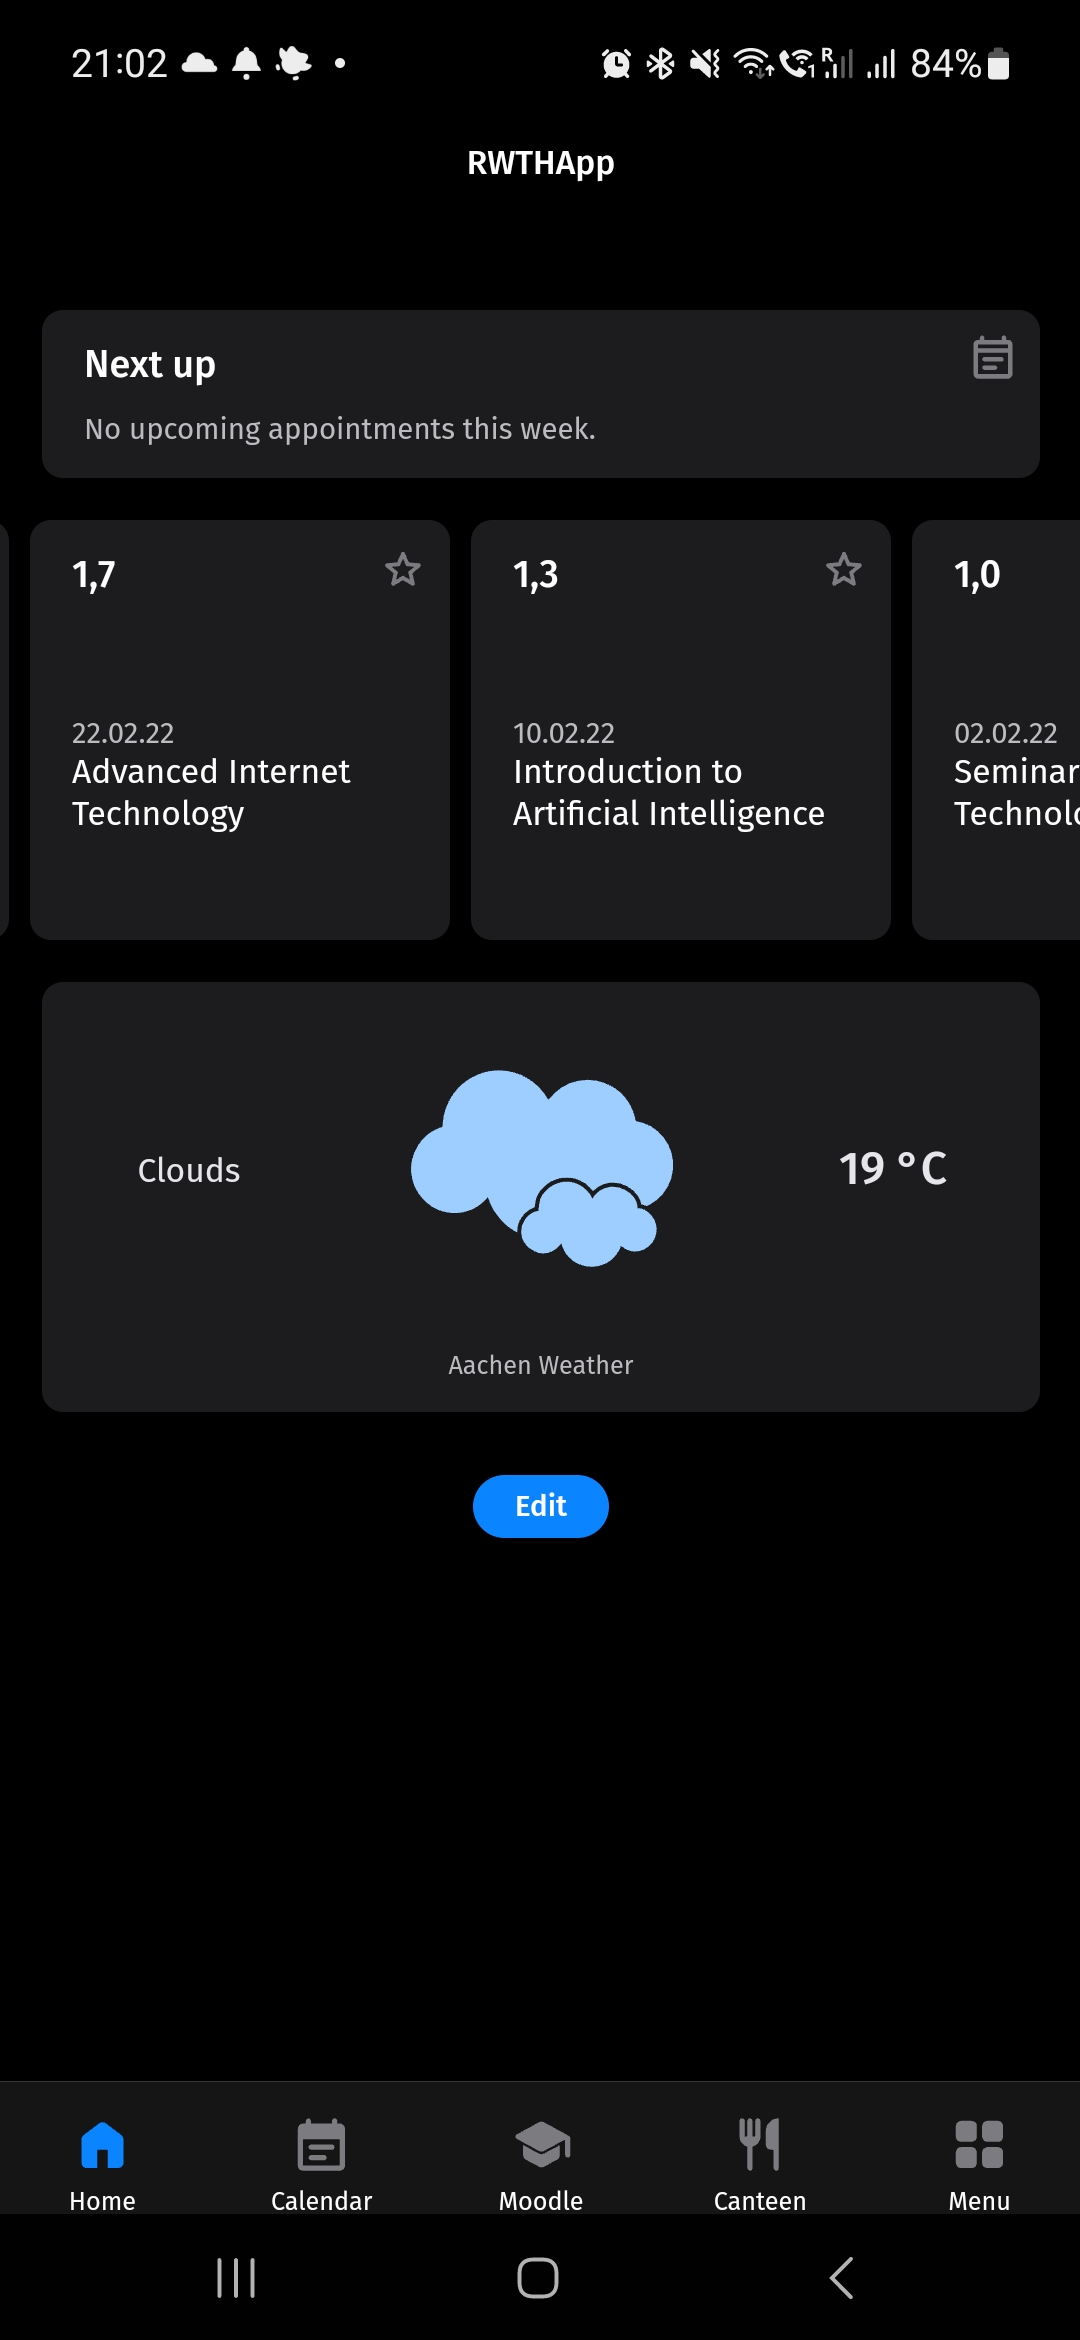
\includegraphics[height=30em]{figures/Screenshot_main_RWTHApp.jpg}
		\caption{This panel is shown on start-up of the app}
		\label{fig:app_main}
	\end{subfigure}
	\hfill
	\begin{subfigure}[T]{0.3\linewidth}
		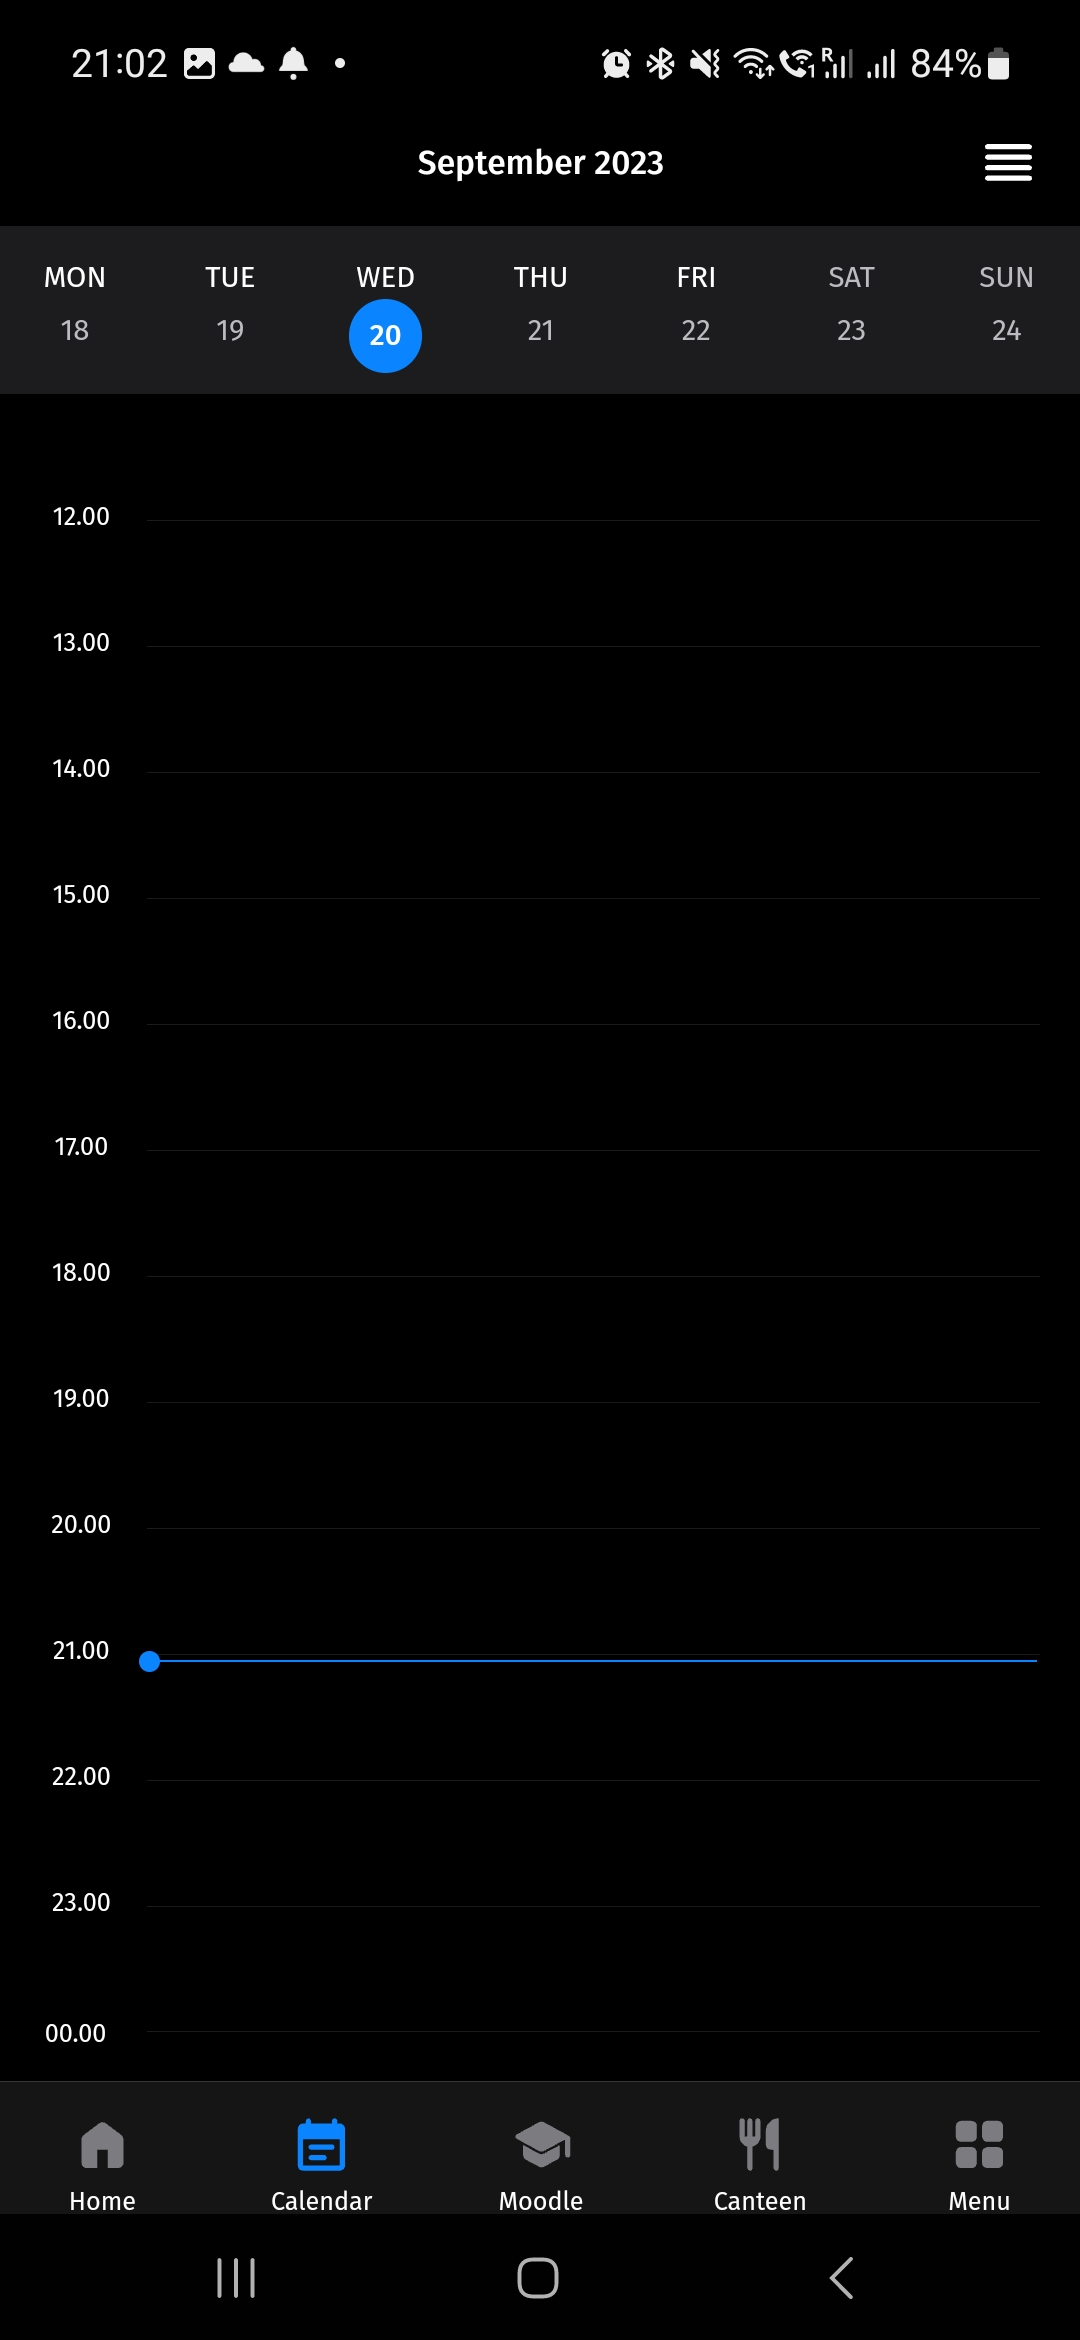
\includegraphics[height=30em]{figures/Screenshot_calender_RWTHApp.jpg}
		\caption{The calender tab shows all assignments that the student has signed up for}
		\label{fig:app_caldener}
	\end{subfigure}
	\hfill
	\begin{subfigure}[T]{0.3\textwidth}
		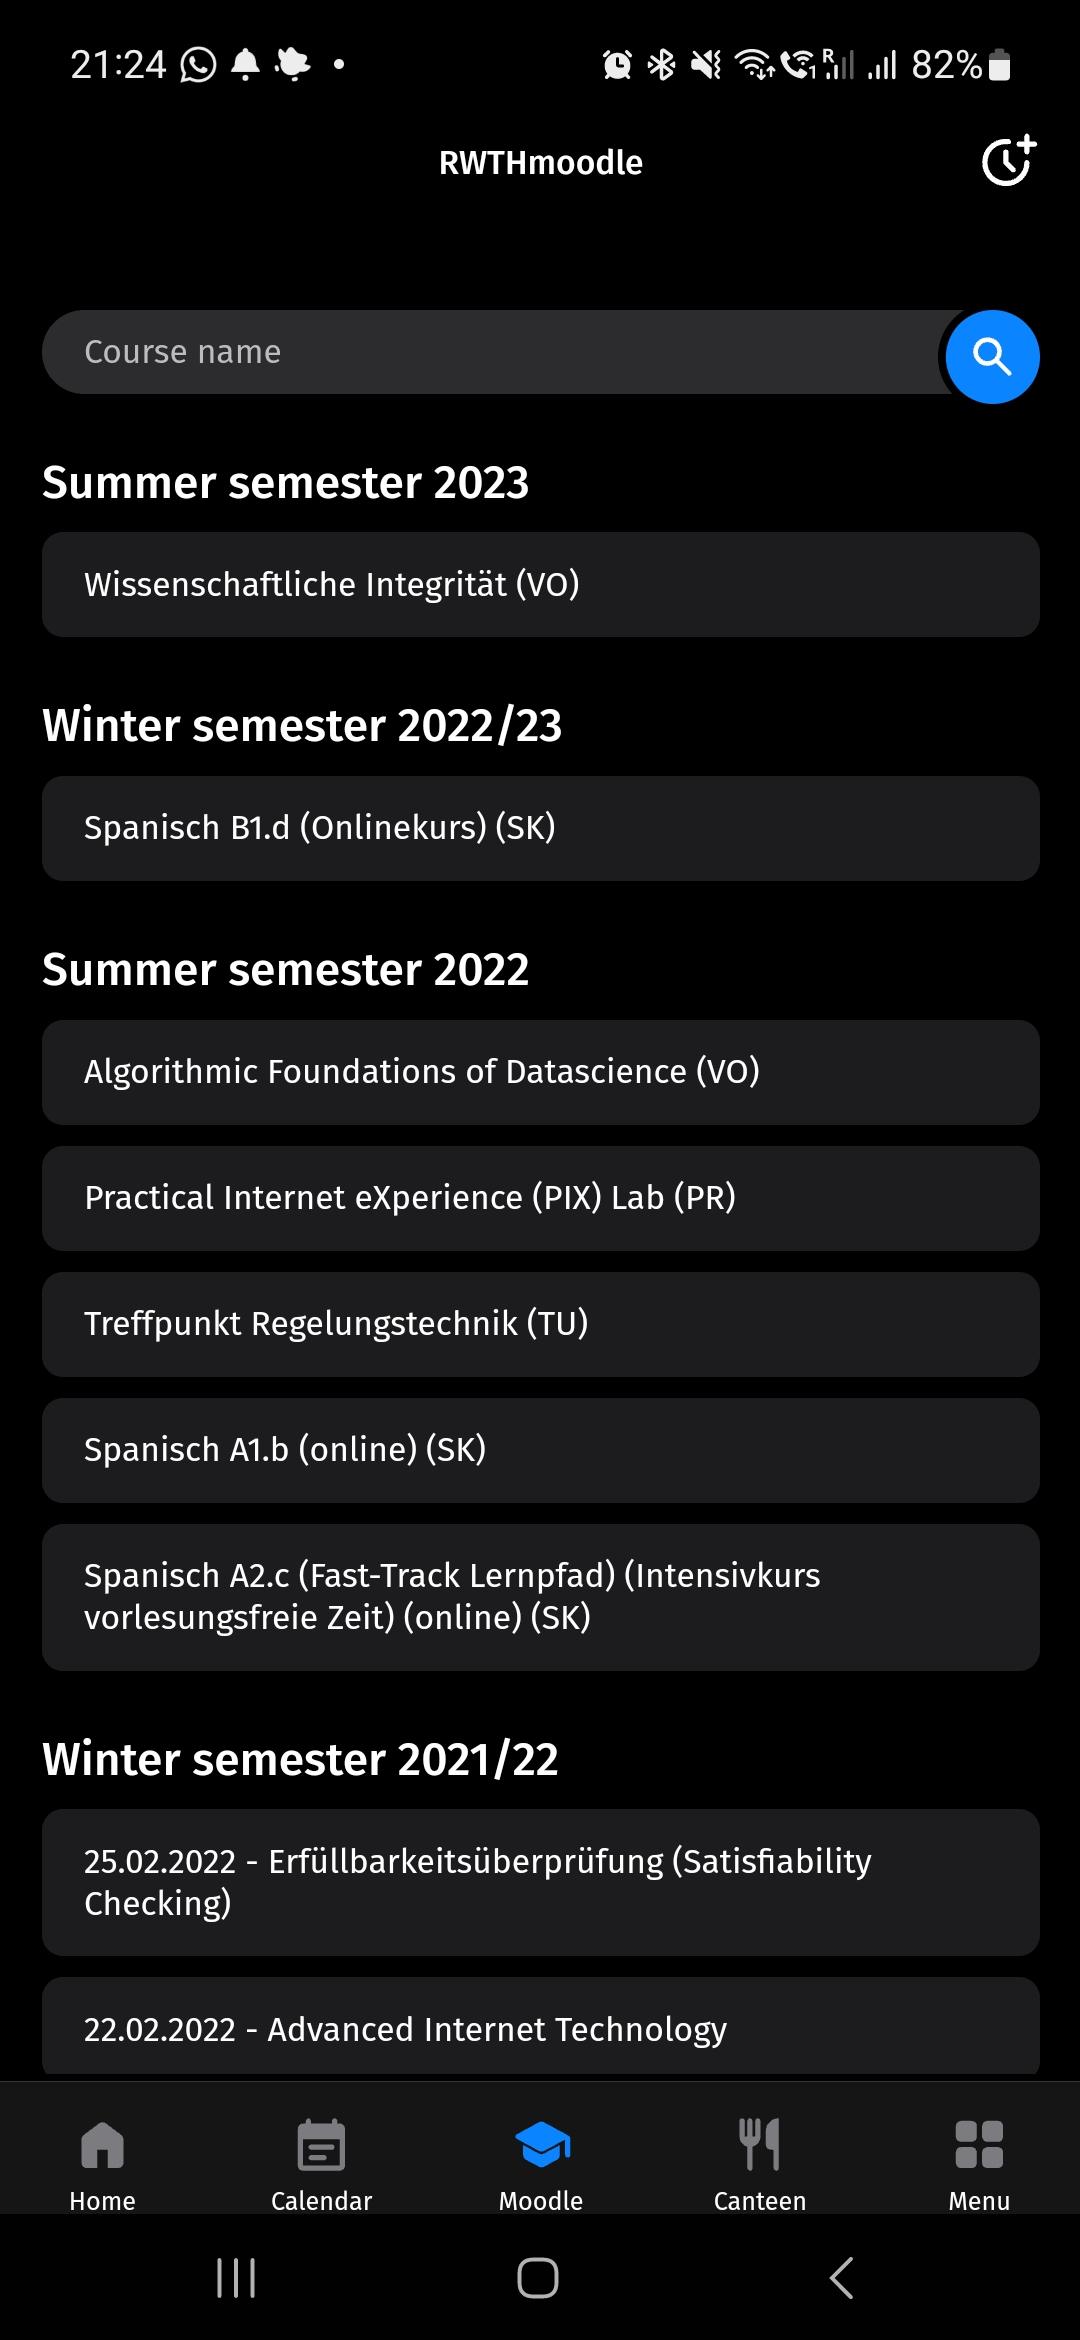
\includegraphics[height=30em]{figures/Screenshot_moodle_RWTHApp.jpg}
		\caption{In the Moodle tab we see all current and past digital classrooms. Furthermore we find links to each classroom and can download items from each class}
		\label{fig:app_moodle}
	\end{subfigure}
	\label{fig:app_1}
\end{figure}

\begin{figure}[t!]
	\centering
	\begin{subfigure}[T]{0.3\textwidth}
		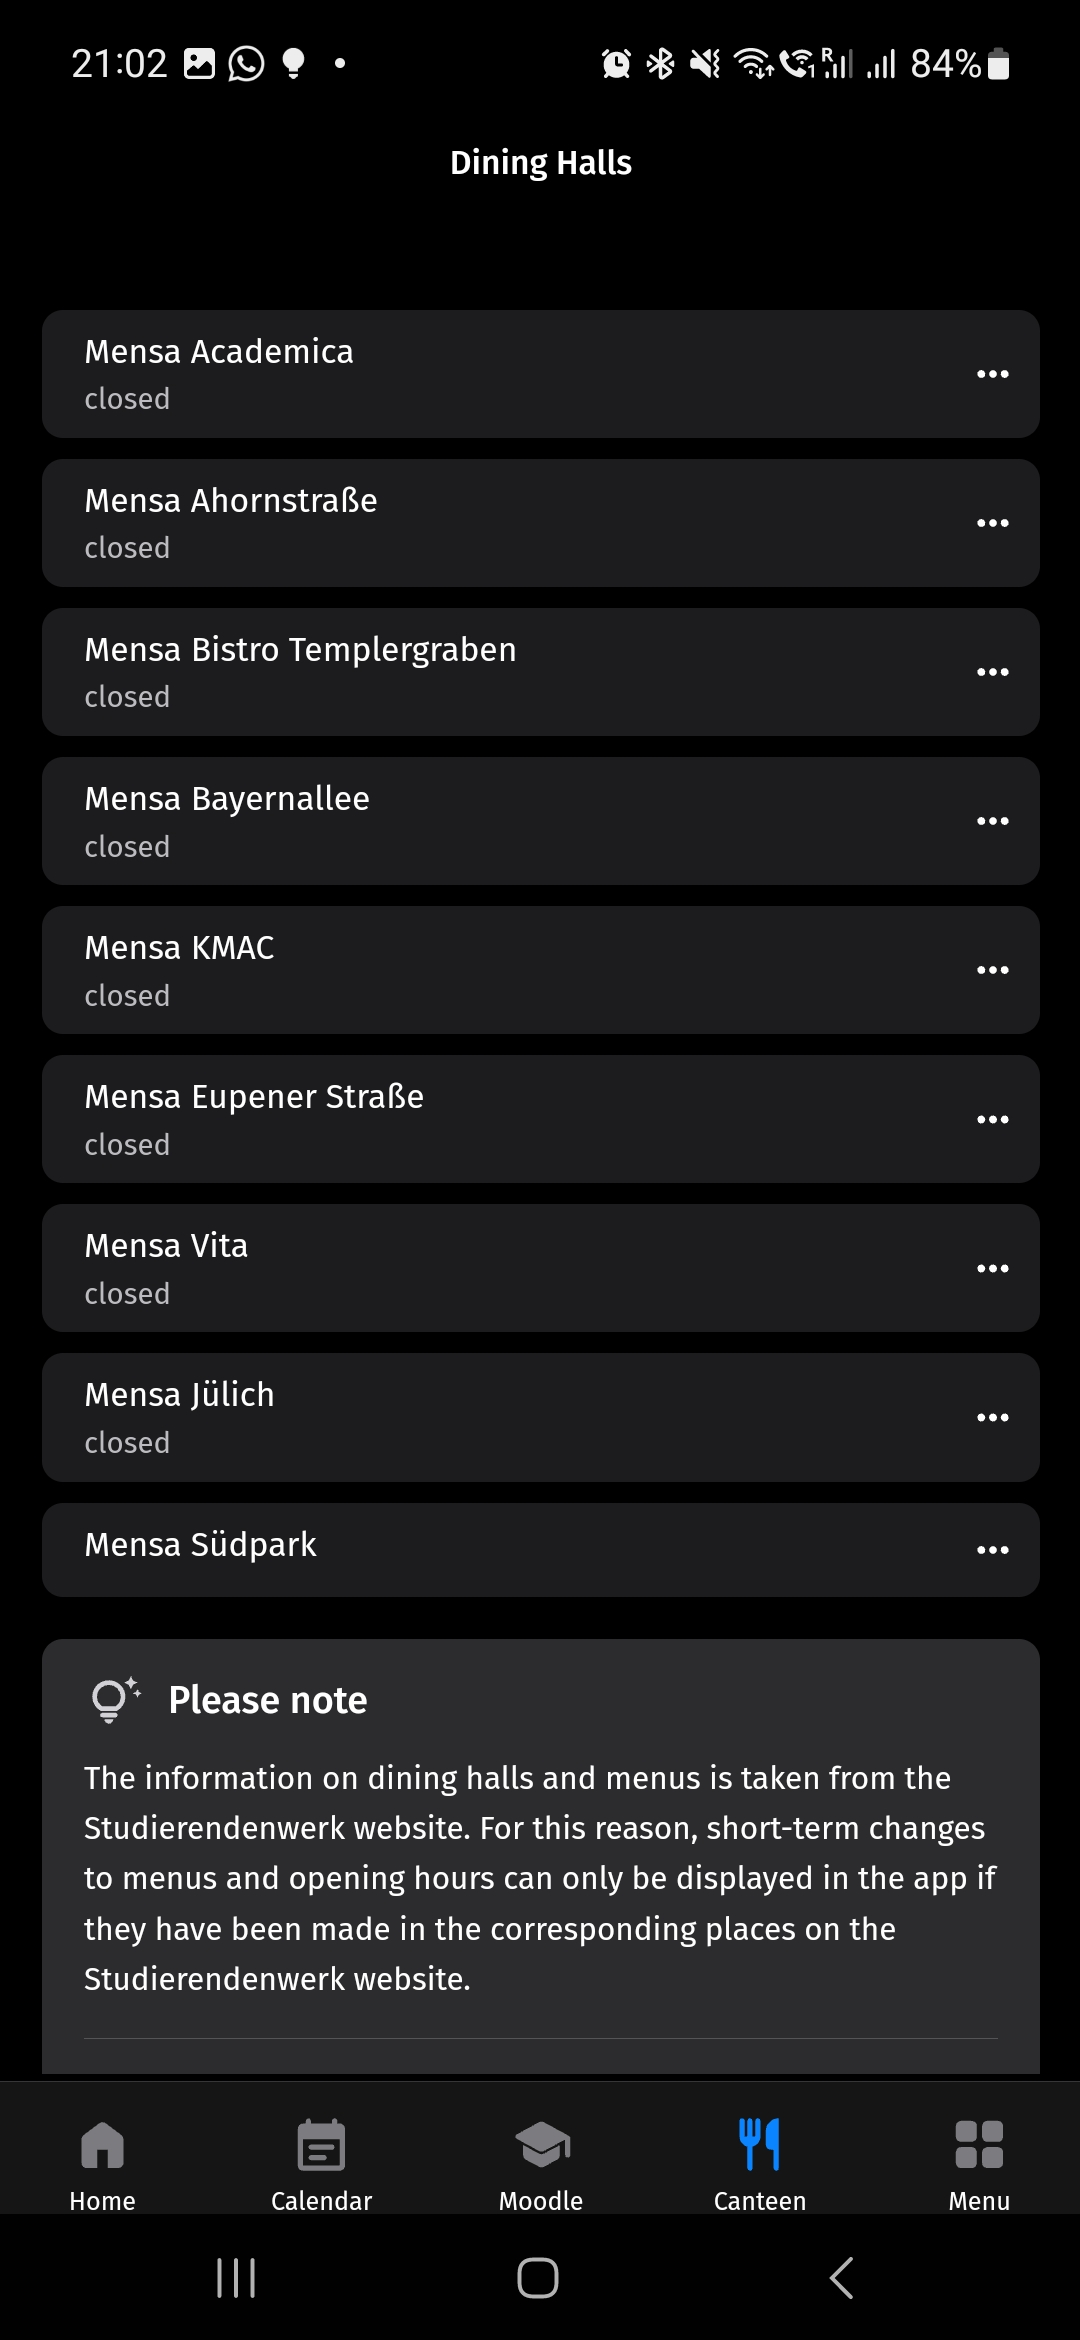
\includegraphics[height=30em]{figures/Screenshot_canteen_RWTHApp.jpg}
		\caption{The Canteen tab shows information on food  served at all university canteens for the current week}
		\label{fig:app_canteen}
	\end{subfigure}
	\hspace{15px}
	\begin{subfigure}[T]{0.3\textwidth}
		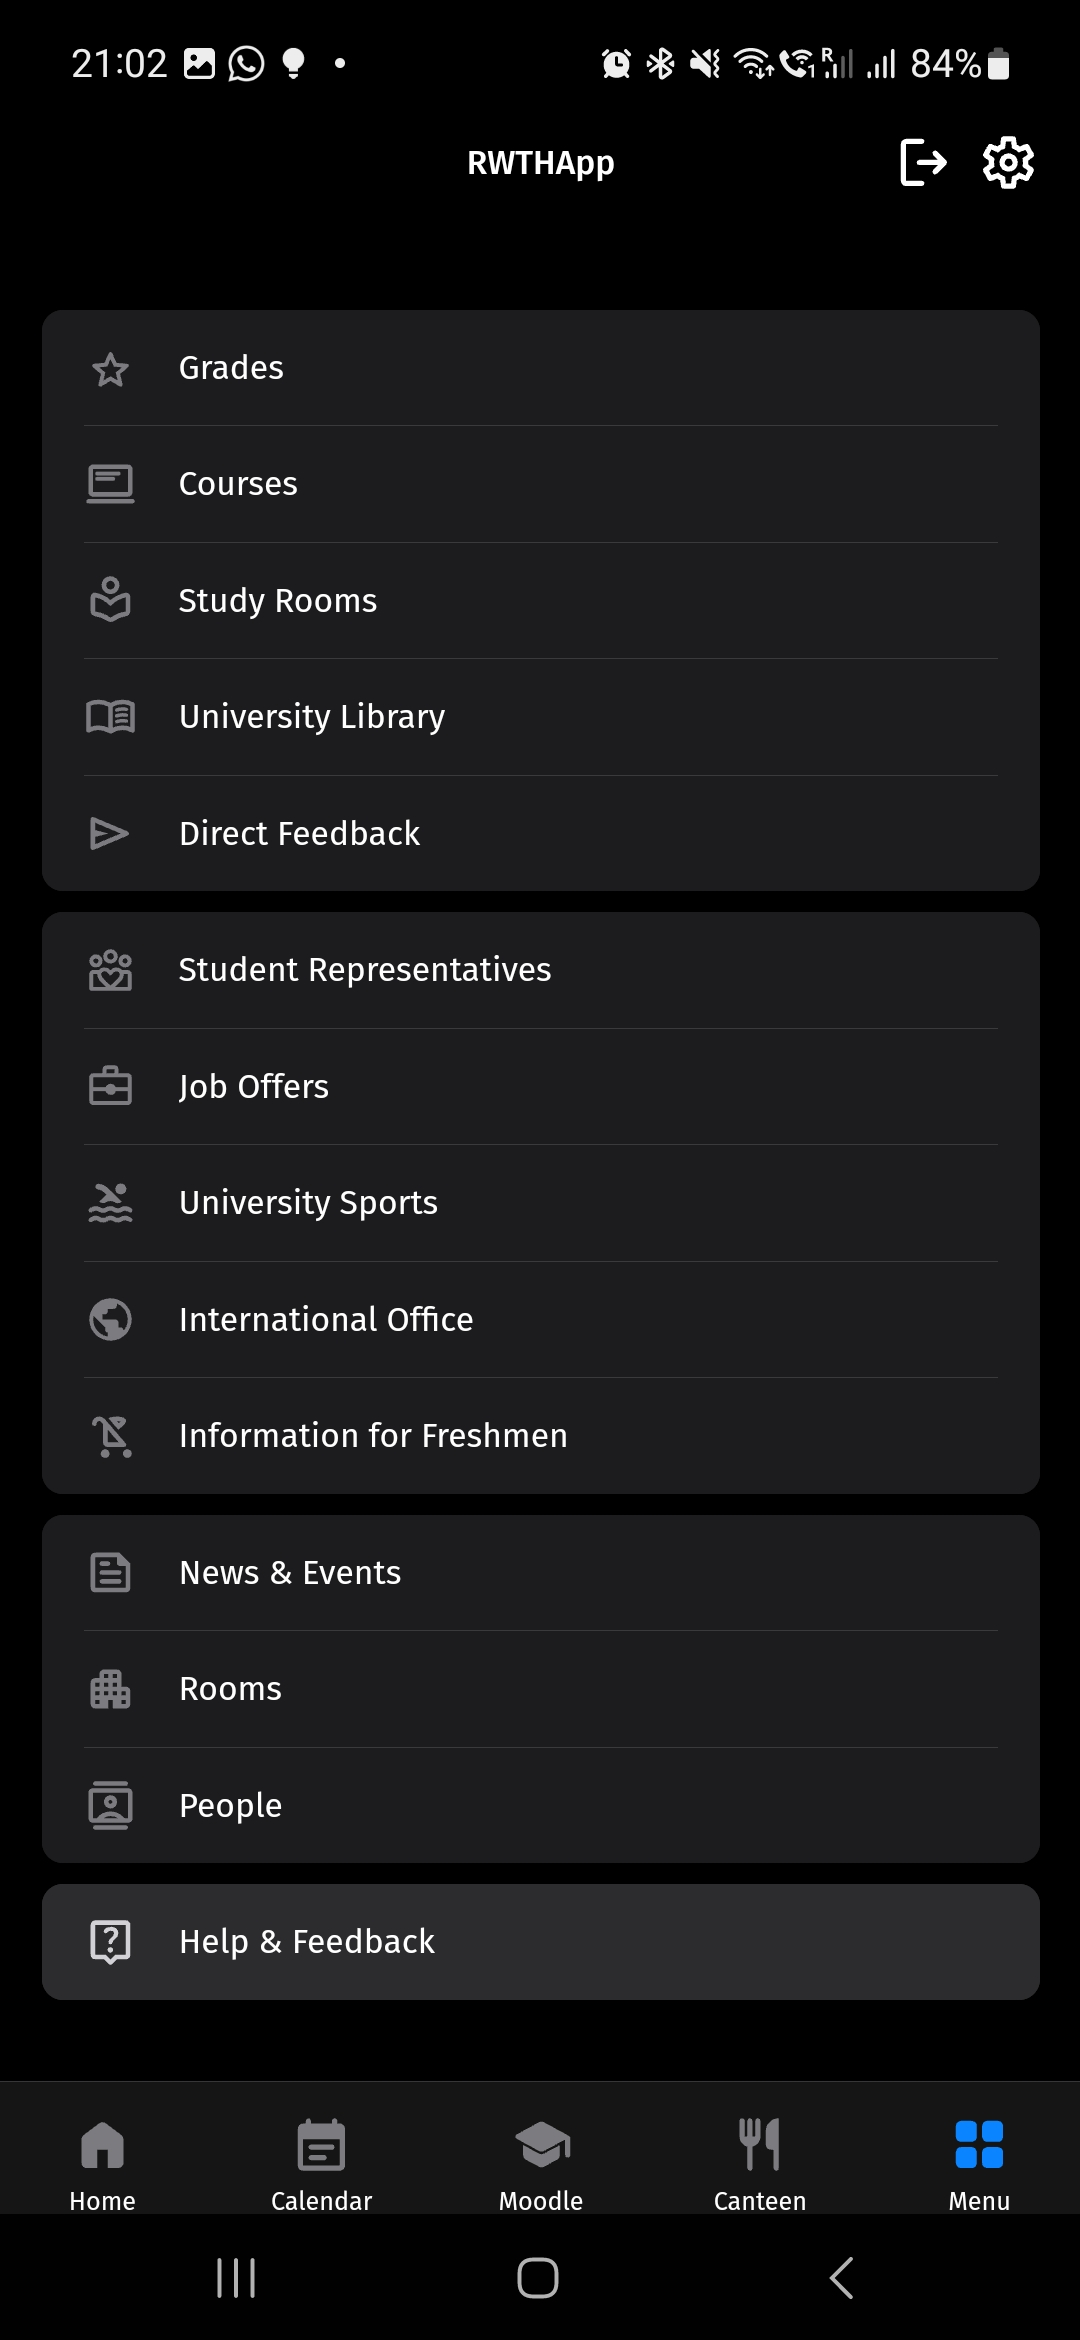
\includegraphics[height=30em]{figures/Screenshot_menu_RWTHApp.jpg}
		\caption{This tab provides quick access to a variety of student services including the library, the sports centre and the international office}
		\label{fig:app_menu}
	\end{subfigure}
	\label{fig_app_2}
\end{figure}

\section{Analysis}
In this analysis we will primarily focus on the WCAG 2.0/2.1 mobile application guidelines. We will pursue a similar structure as in our analysis of the webpage.
\subsection*{Perceivable}
The app adapts well to screen sizes and uses OS-level settings for font size. There is no built in zoom-feature, but OS-level zoom works and the app is generally designed to be easy to read. It comes with a built in dark-mode that can be activated by the user and helps increase contrast levels throughout the app.

\subsection*{Operable}
The interface is well designed to prevent mis-clicks as different items are fairly large in size and feature clear boundaries to the environment. To our knowledge, the app makes no use of \textsl{device manipulation gestures} such as shaking or tilting, other than entering a landscape mode when tilted completely sideways. This landscape mode rearranges content items in a sensible manor in a side-by-side or fit-to-screen stretch fashion. All functionality stays usable and operable, though to reach to the far left end (in landscape mode) the user my find it easier to use a second hand.
In portrait mode, all items in the menu bar and most content items are easy to reach, with the only exception being the top bar in the calender. The user might need to reposition their hand to reach for the leftmost weekdays.

\subsection*{Understandable}
The overall layout of the app consist of a menu bar at the bottom that stays visible throughout all pages of the app. In the top, we find the headline for each page. The  majority of space is comprised of the content of each page. This scheme is consistent across all pages.
Content may be scrollable, though the top heading and bottom menu stay in the same place while main content scrolls up and down.
As we alluded to in the section before, the lanscape mode seamlessly works with all features and keeps the layout structure.
The static elements of the page, such as menu-bar and top-heading help users with impaired vision to navigate more easily across the app as they provide a point of reference.
The graphic style used to indicate intractable items is based on a "button design". Ever item a user can interact with has a button shaped, rounded box and is visually distinct from its background.
In case of the menu bar, there are icons and text indicating the purpose of a menu item.

\subsection*{Robustness}
Without access to the source code it is difficult to determine robustness factors of this app. There are no special support features for people with disabilities other than the standard OS-level features such as zoom, font size, etc.
As there is no need for the user to enter any data, no keyboard is required to use the app. 
As we neither could not find any scaling, or adaption issues on our device nor have we heard of problems from other users, we suspect, that the app is well build to run seamless on a large variety of devices and screen sizes. It is to note though, that we have no actual proof for this claim as we did not perform a survey across different users.

\subsection*{Conclusion}
From our visual analysis, we decide this app to be very well build to high standards of accessibility. We could not find any major flaws while exploring the app in the context of accessibility.













